%********************************************************************
% Appendix
%*******************************************************
% If problems with the headers: get headings in appendix etc. right
%\markboth{\spacedlowsmallcaps{Appendix}}{\spacedlowsmallcaps{Appendix}}
\chapter{Appendix}
\addtocontents{toc}{\protect\setcounter{tocdepth}{0}}

\renewcommand{\thefigure}{A\arabic{figure}}
%\section{Supplementary information}
\setcounter{figure}{0}
%%%%%%%%\counterwithin{figure}{section}
\section{Statistics of Southern Ocean carbon sink}
\begin{figure}[h!]
        \myfloatalign
        \captionsetup[subfigure]{justification=centering}
        \subfloat[Southern Ocean sea-air CO$_2$ flux \text{[PgC/yr]}]
        {\label{fig:SOCS_temporal_gaussian-a}%
        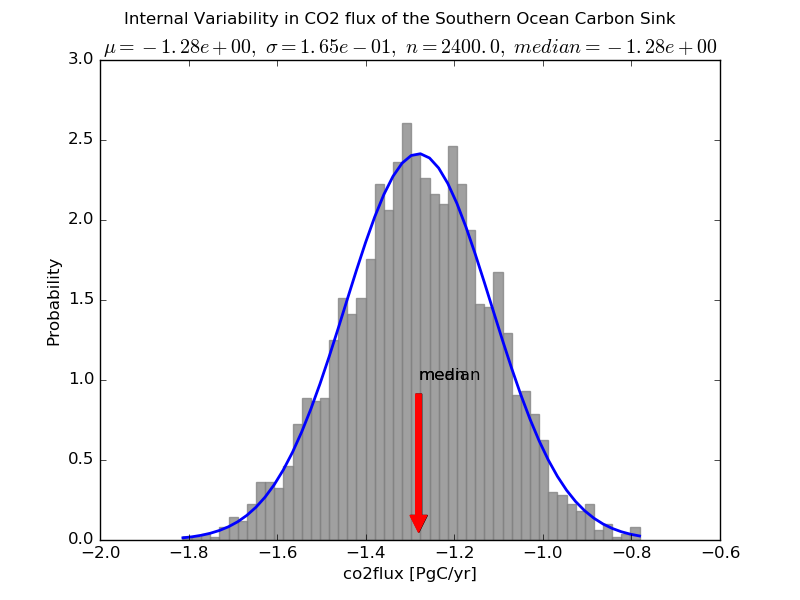
\includegraphics[scale=.53,trim=0cm 0cm 0cm 1cm,clip]{new_SOCS_co2flux_Distribution_n24.png}} \quad
        \subfloat[Southern Ocean sea-air CO$_2$ flux of a single grid cell \text{[kgC m$^{-2}$s$^{-1}$]}]
        {\label{fig:SOCS_temporal_gaussian-b}%
         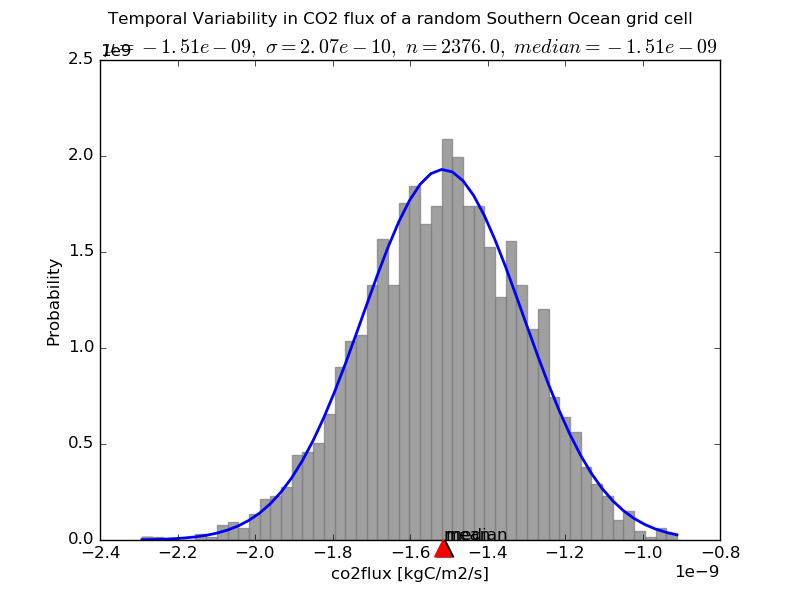
\includegraphics[scale=.53,trim=0cm 0cm 0cm 1cm,clip]{new_SO_co2flux_Spatial_Distribution_n24.png}} \\
        \caption{Propability distribution function of the annual sea-air CO$_2$ flux in the Southern Ocean in ensemble space and temporal space between 1980-2004: (a) field sum over 35-90$^\circ$S and (b) in a random grid cell.} \label{fig:SOCS_temporal_gaussian}
\end{figure}

\clearpage
\section{CO$_2$ flux trends}
\begin{figure}[h!]
	\topinset{\textbf{*}}{\topinset{\textbf{*}}{\topinset{\textbf{*}}{\topinset{\textbf{*}}{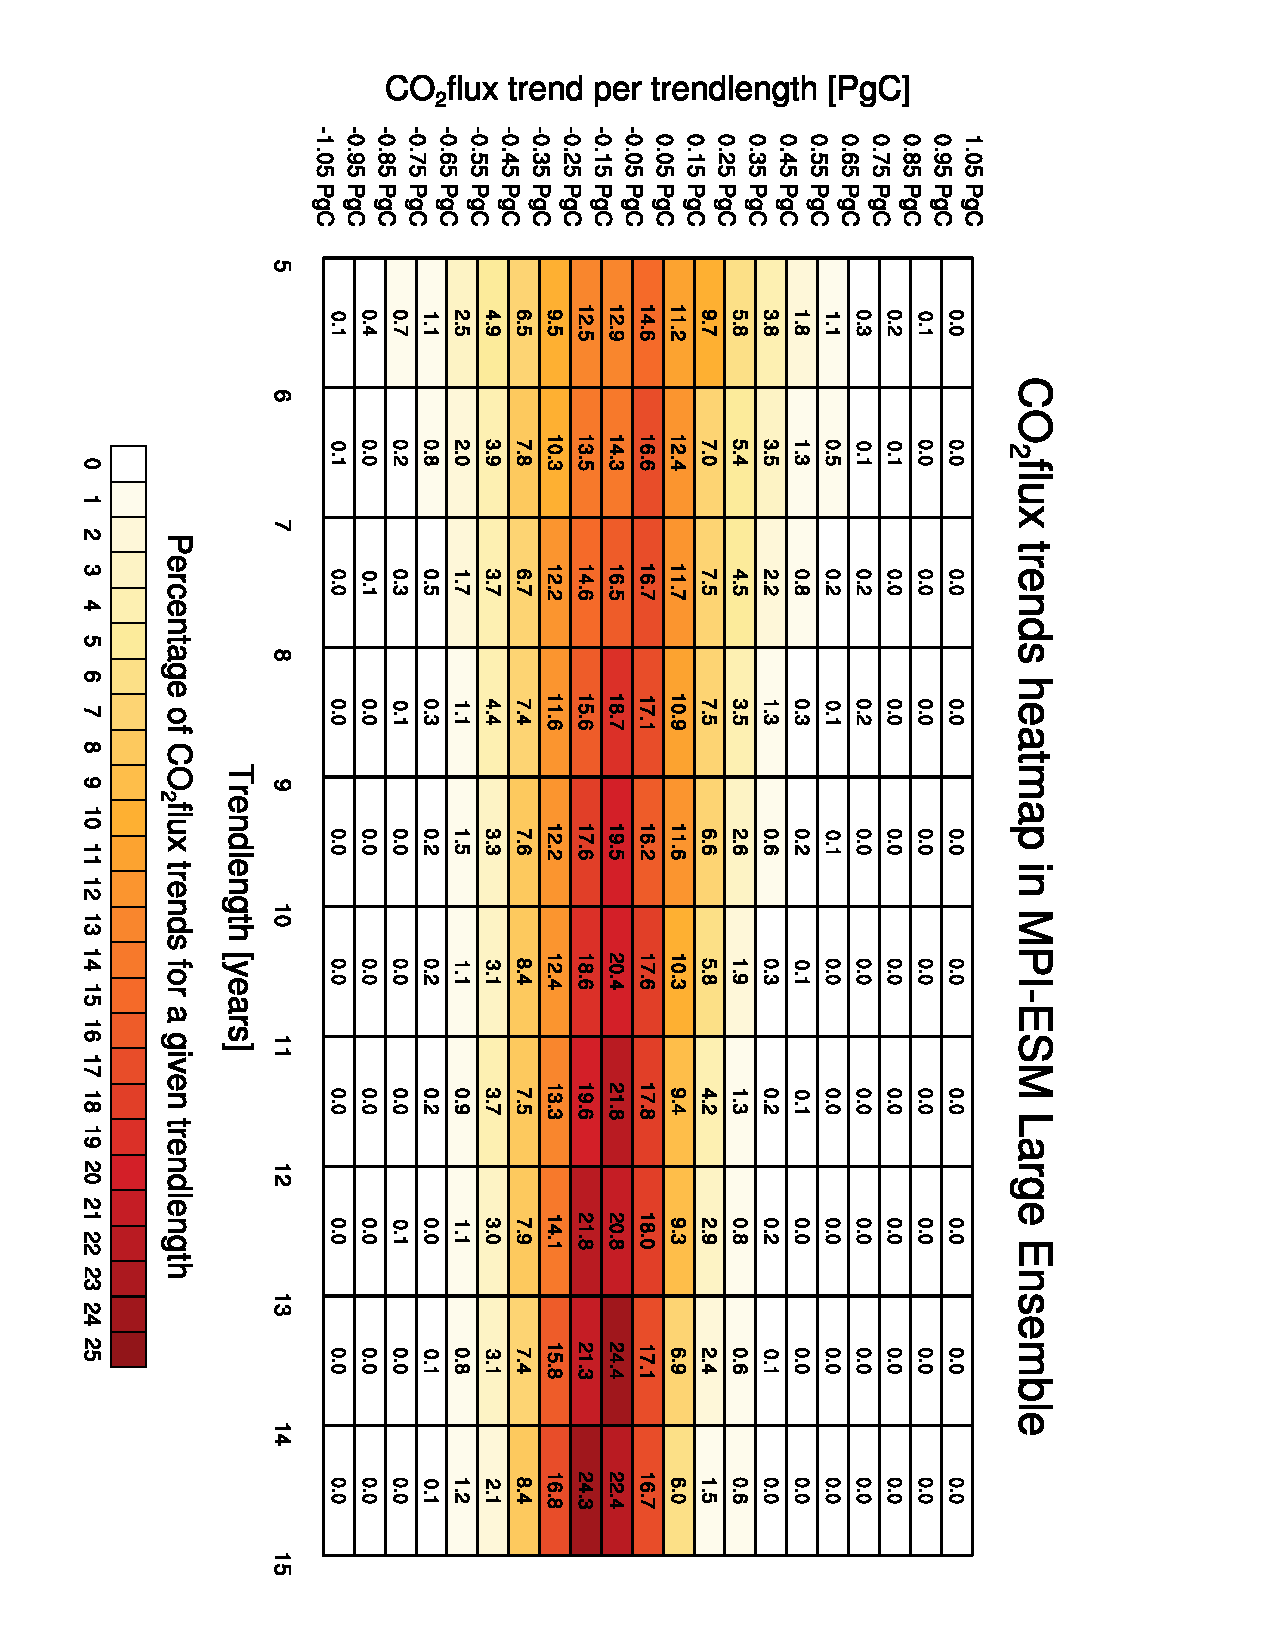
\includegraphics[scale=.75,angle=0,trim=1.4cm 1.3cm 1cm 2cm,clip]{heatmap_not_de-ens-trended.pdf}}{11.1cm}{9.1cm}}{7.75cm}{9.1cm}}{7.75cm}{4.8cm}}{11.1cm}{4.4cm} % from gfx folder
	%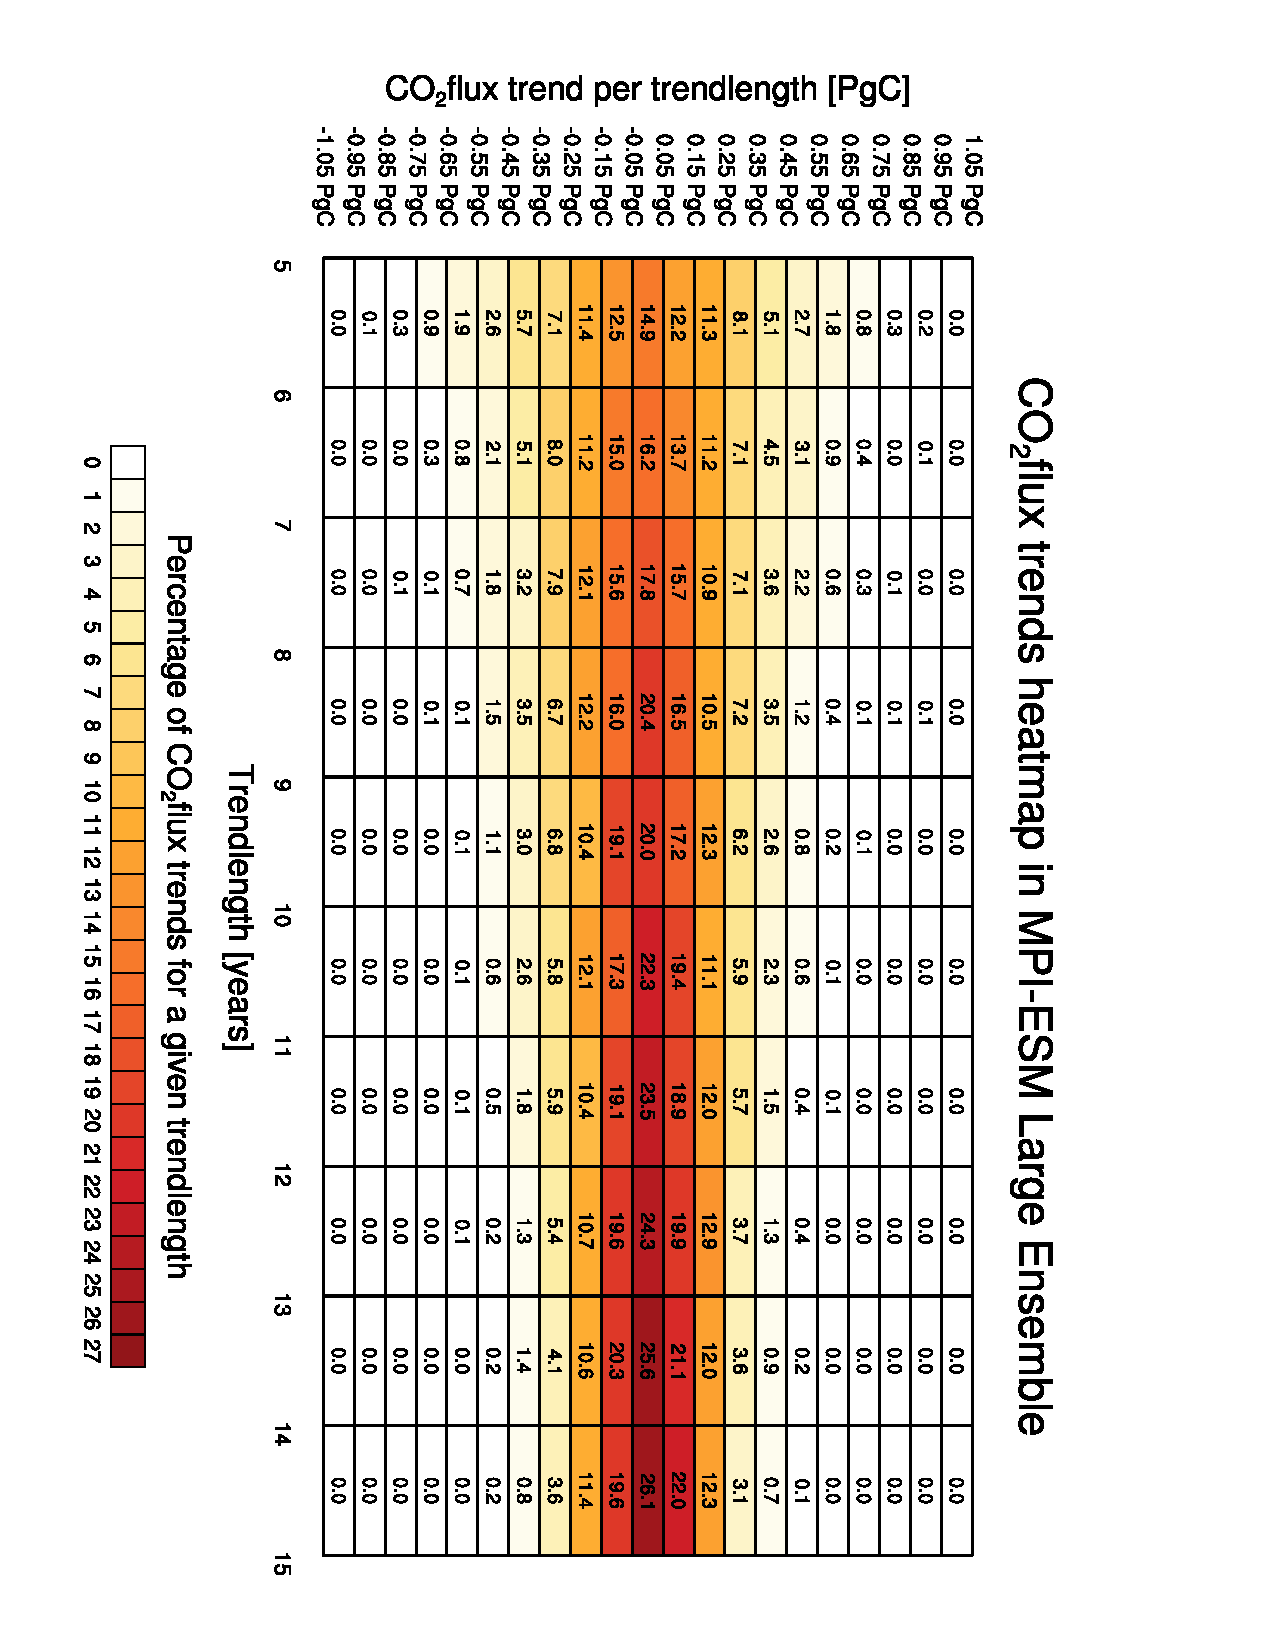
\includegraphics[scale=.64,angle=90,trim=1.3cm 1.3cm 5cm 1cm,clip]{heatmap_de-ens-trended.pdf} % from gfx folder
\caption{Southern Ocean carbon sink trends per trend length; * indicate the strongest 8-year and 10-year trends in \ac{SOM-FFN}}
	\label{fig:heatmap}
\end{figure}

\begin{figure}[h!]
	%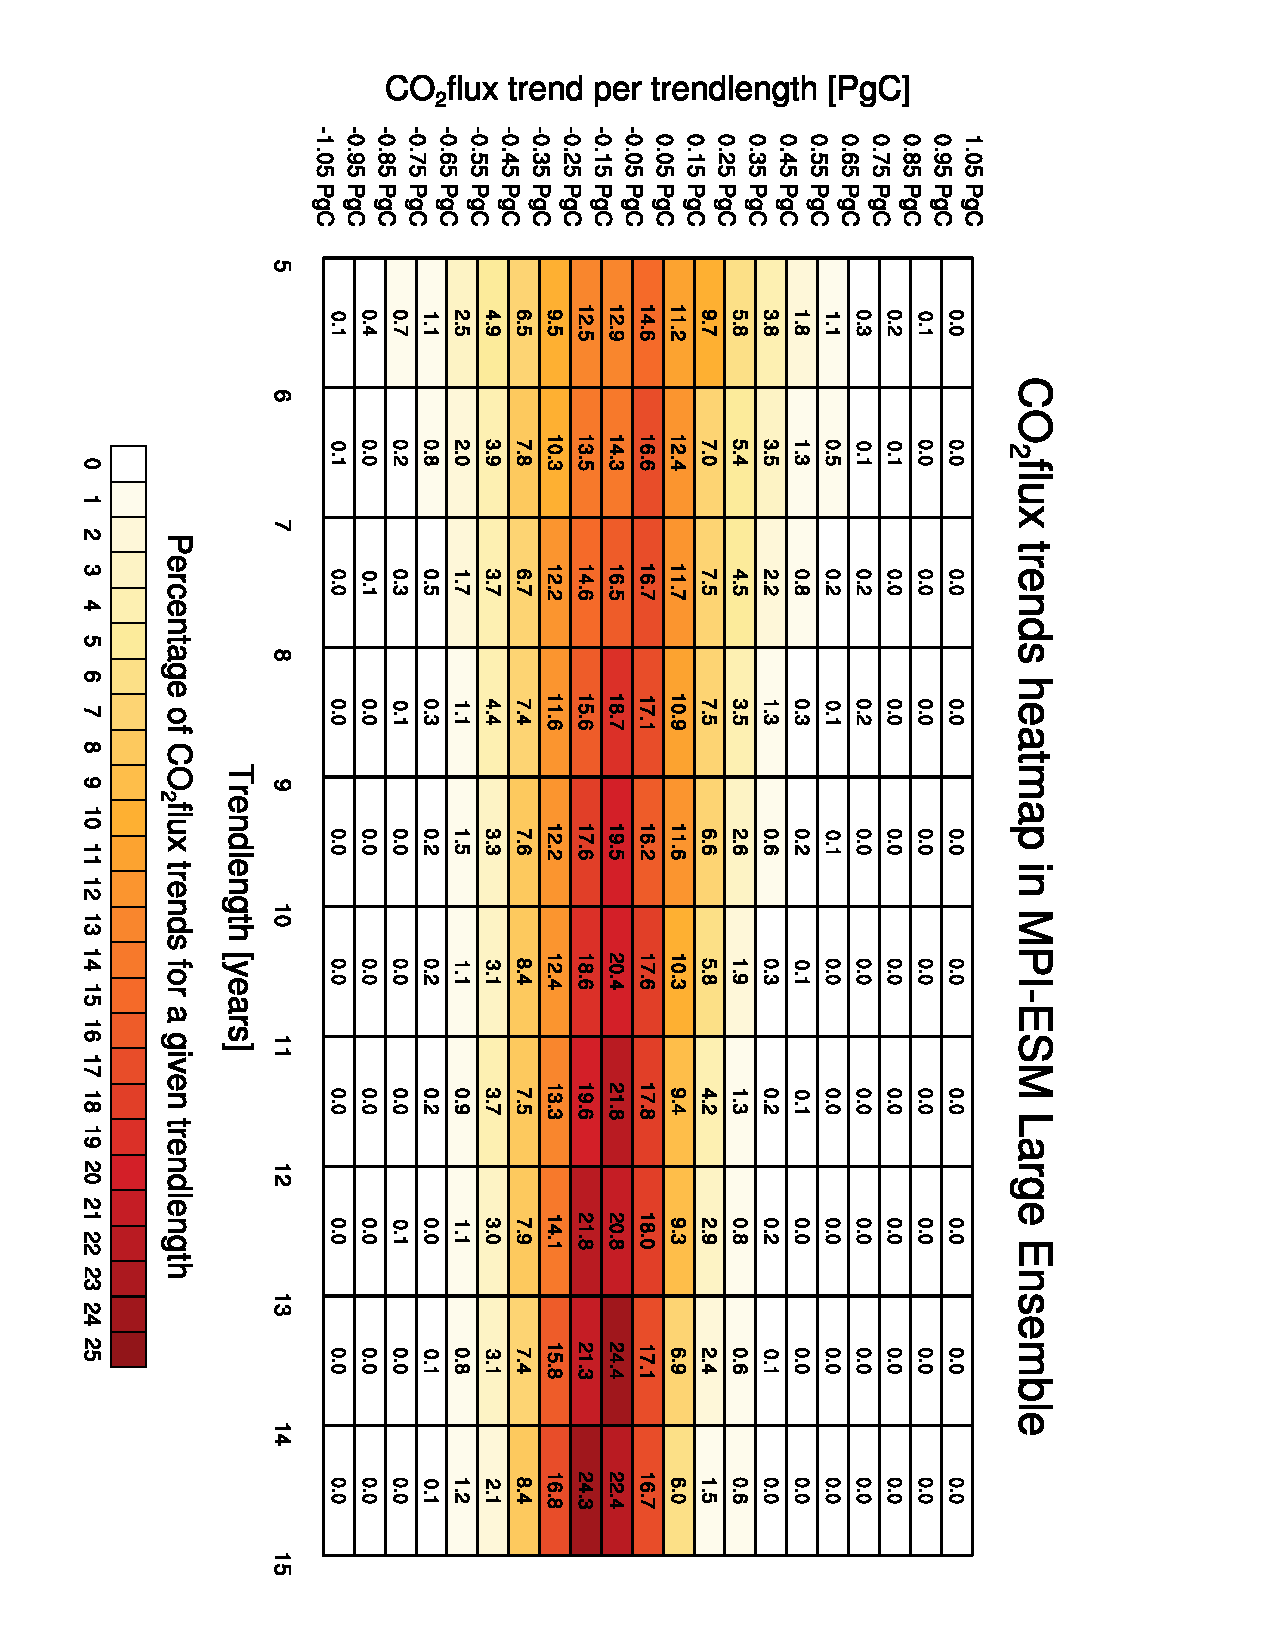
\includegraphics[scale=.75,angle=0,trim=1.4cm 1.3cm 1cm 1cm,clip]{heatmap_not_de-ens-trended.pdf} % from gfx folder
	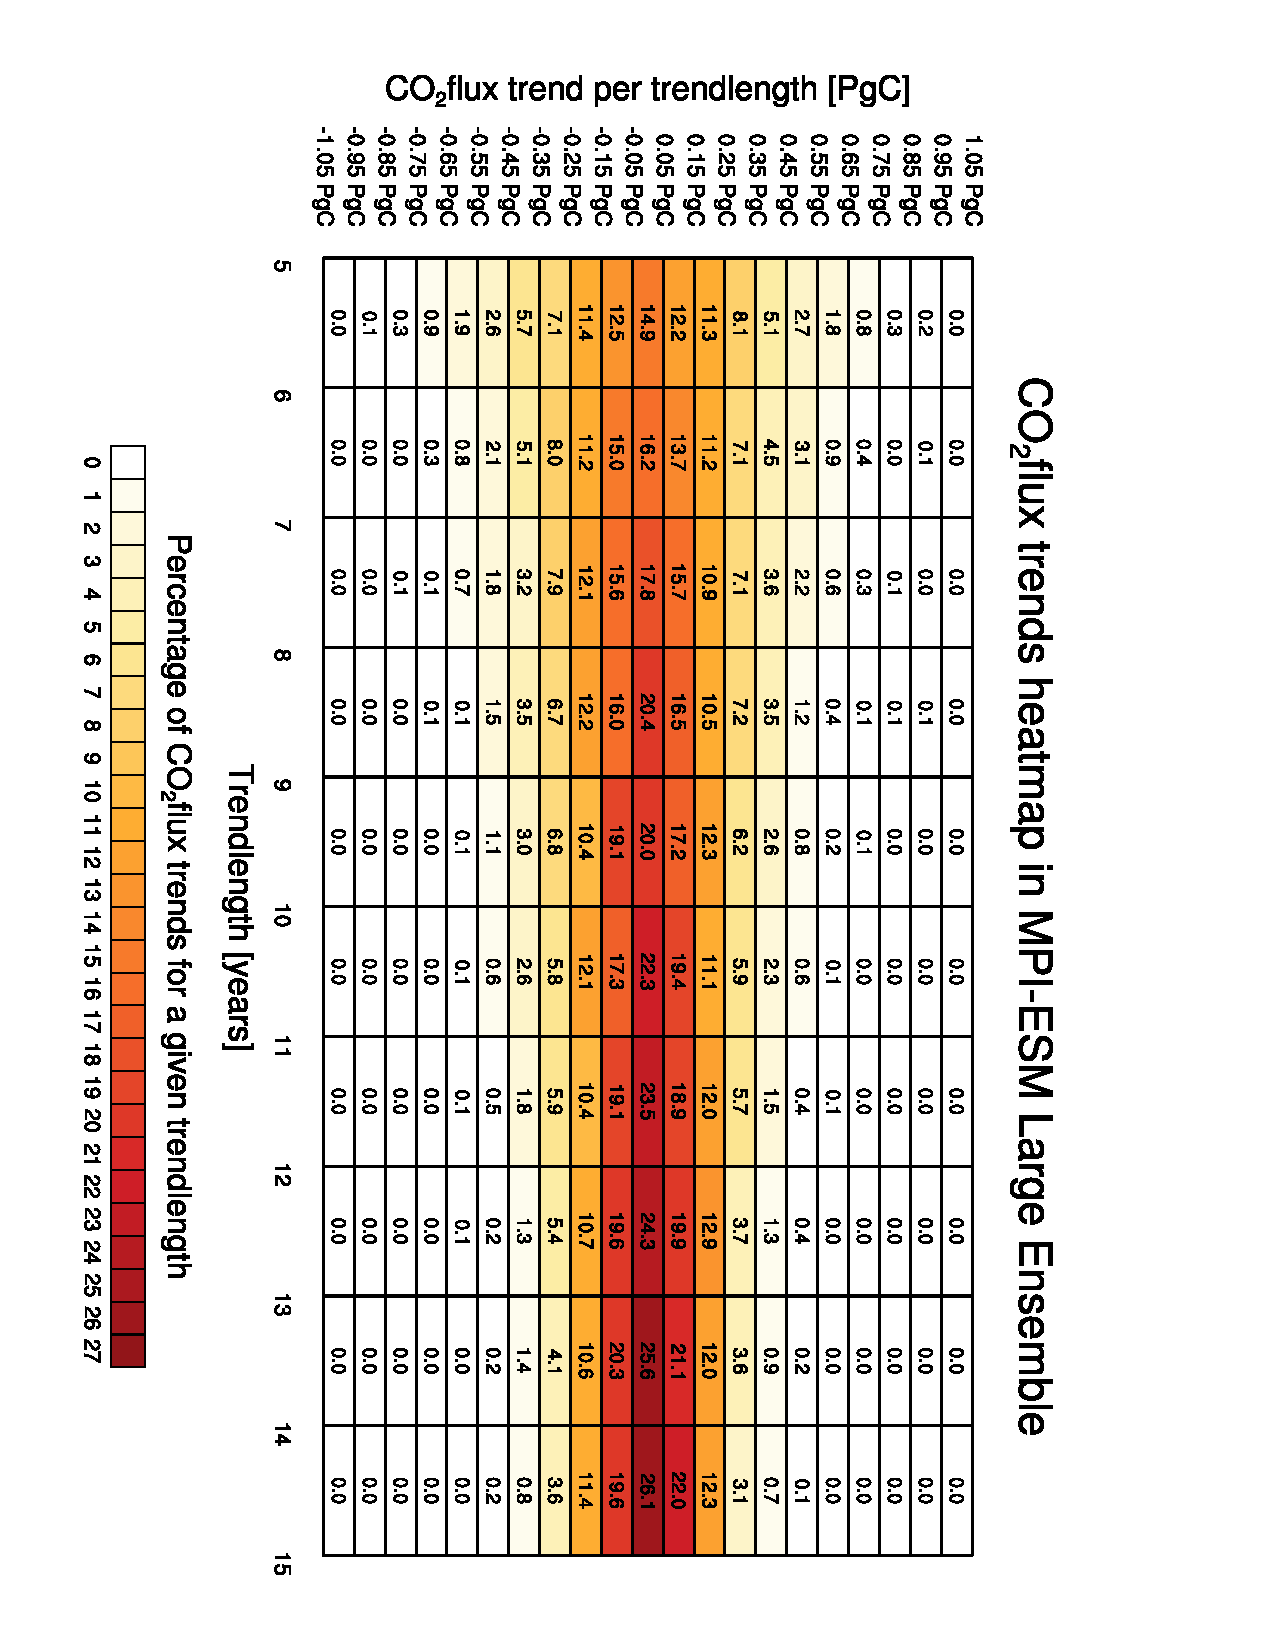
\includegraphics[scale=.75,angle=0,trim=1.4cm 1.3cm 1cm 1cm,clip]{heatmap_de-ens-trended.pdf} % from gfx folder
\caption{Southern Ocean carbon sink trends per trend length; corrected for forced trend}
	\label{fig:heatmap_detrended}
\end{figure}



\clearpage
\section{Model evaluation additum}
\begin{figure}[bth]
        \myfloatalign
        \subfloat[\acs{MPI-ESM} surface \acs{DIC} ensemble \text{      }  \text{      } mean \text{[mmol C m$^{-3}$]}]
        {\label{fig:SOCS_comp_DIC-a}%
       \includegraphics[scale=.66,page=2,trim=1.3cm 13.3cm 12.1cm 6.5cm,clip]{Overview_SO_nutrient_comparison.pdf}} %\quad
        \subfloat[\acs{GLODAP}v2 surface \acs{DIC} mean \text{      }  \text{      } \text{      }  \text{      } \text{      }  \text{      }\text{[mmol C m$^{-3}$]}]
        {\label{fig:SOCS_comp_DIC-b}%
         \includegraphics[scale=.66,page=2,trim=9.4cm 13.3cm 2.1cm 6.5cm,clip]{Overview_SO_nutrient_comparison.pdf}} \\
       \caption{Spatial distribution of the climatology of surface \acf{DIC}: (a) \acs{MPI-ESM LE} climatology, (b) \acf{GLODAP} Version 2 climatology \citep{GLODAPv2}.} \label{fig:SOCS_comp_DIC}
\end{figure}

\begin{figure}[bth]
        \myfloatalign
        \subfloat[\acs{MPI-ESM} surface phosphate ensemble \text{      }  \text{      } mean \text{[mmol P m$^{-3}$]}]
        {\label{fig:SOCS_comp_phosph-a}%
       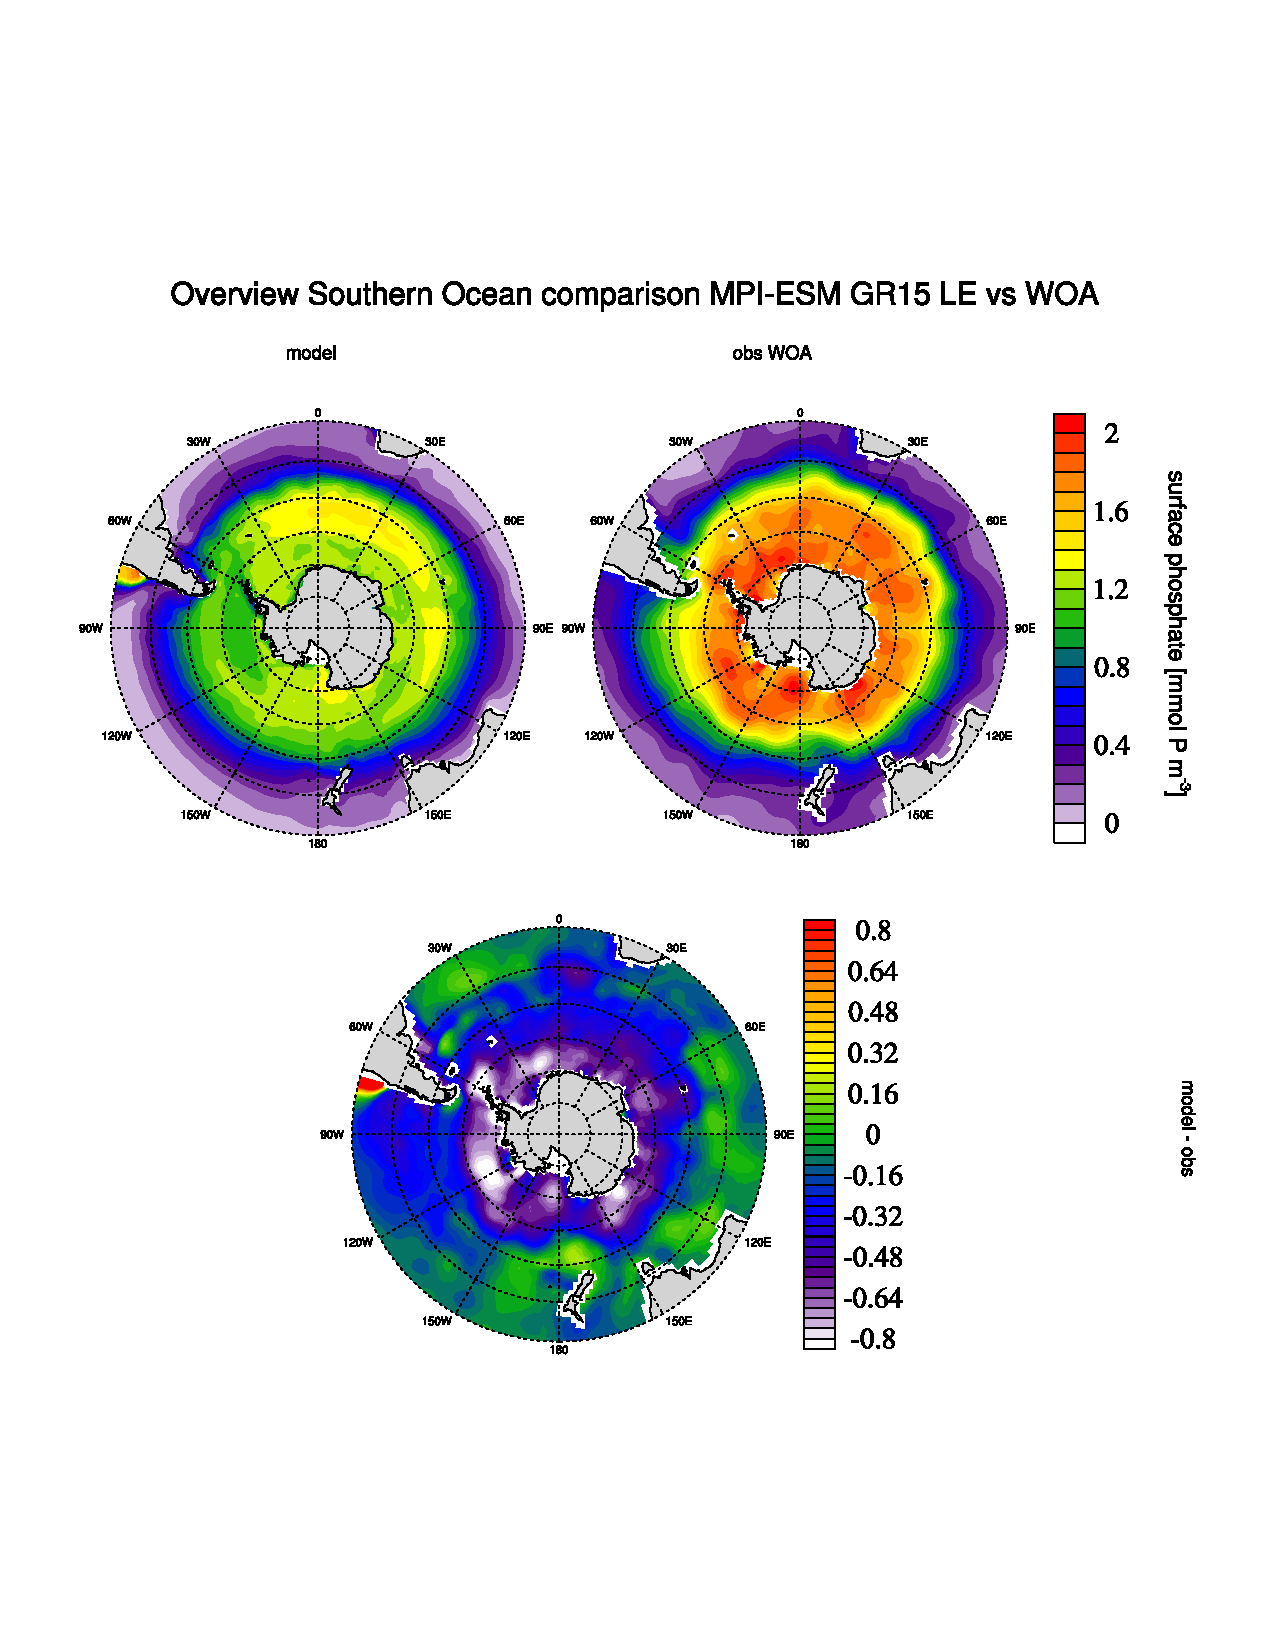
\includegraphics[scale=.66,page=1,trim=1.3cm 13.3cm 12.1cm 6.5cm,clip]{Overview_SO_nutrient_comparison.pdf}} %\quad
        \subfloat[\acs{WOA} surface phosphate mean \text{      }  \text{      } \text{      }  \text{      } \text{      }  \text{      }\text{[mmol P m$^{-3}$]}]
        {\label{fig:SOCS_comp_phosph-b}%
         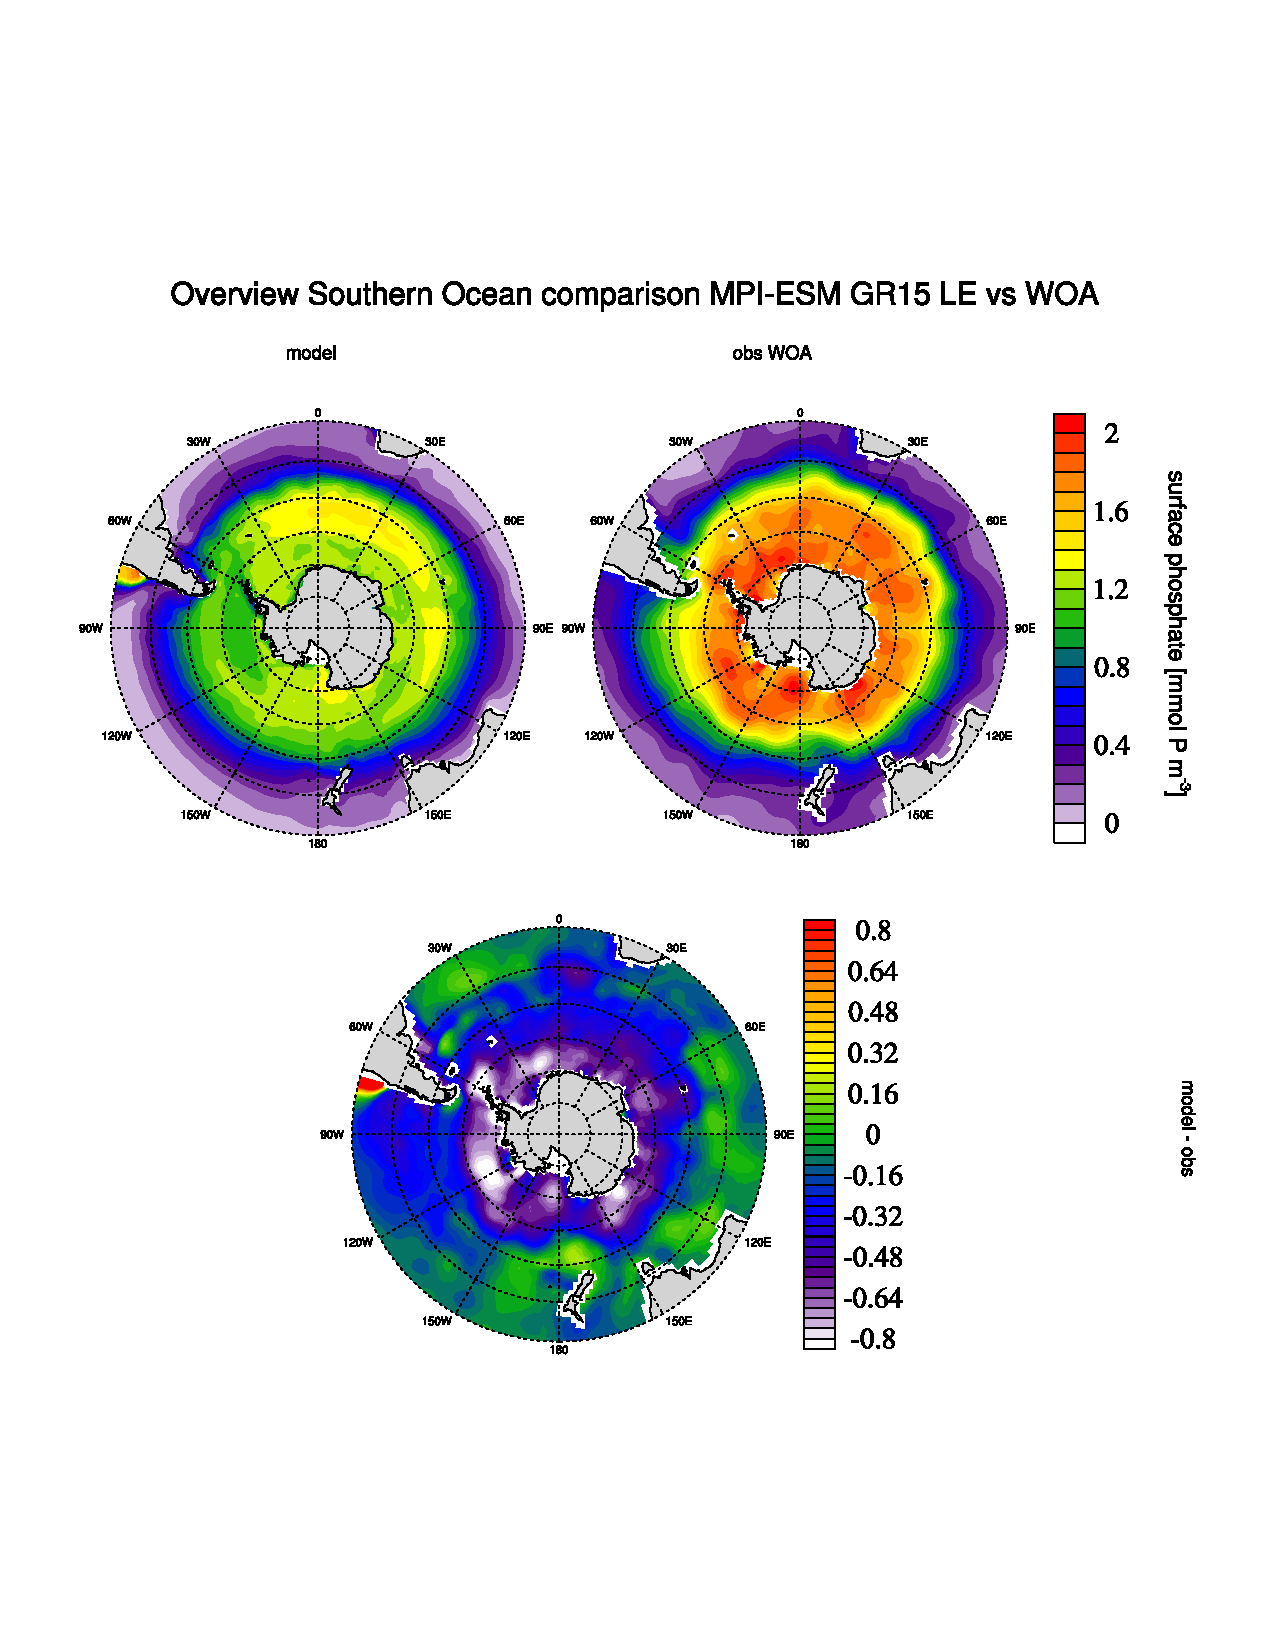
\includegraphics[scale=.66,page=1,trim=9.4cm 13.3cm 2.1cm 6.5cm,clip]{Overview_SO_nutrient_comparison.pdf}} \\
       \caption{Spatial distribution of the climatology of surface phosphate: (a) \acs{MPI-ESM LE} climatology, (b) \acf{WOA} climatologicy \citep{WOA2013}.} \label{fig:SOCS_comp_phosph}
\end{figure}

\begin{figure}[bth]
        \myfloatalign
        \subfloat[\acs{MPI-ESM} \acs{SST} ensemble mean \text{[$^\circ$C]}]
        {\label{fig:SOCS_comp_SST-a}%
       \includegraphics[scale=.66,page=2,trim=1.3cm 13.3cm 12.1cm 6.5cm,clip]{Overview_SO_MPIOM_comparison.pdf}} %\quad
        \subfloat[\acs{WOA} \acs{SST} mean \text{[$^\circ$C]}]
        {\label{fig:SOCS_comp_SST-b}%
         \includegraphics[scale=.66,page=2,trim=9.4cm 13.3cm 2.1cm 6.5cm,clip]{Overview_SO_MPIOM_comparison.pdf}} \\
       \caption{Spatial distribution of the climatology of \acf{SST}: (a) \acs{MPI-ESM LE} climatology, (b) WOCE climatology \citep{WOCE}.} \label{fig:SOCS_comp_SST}
\end{figure}

\clearpage
\section{Thermal separation by seasons}
\subsection{Positive CO$_2$ flux trend}

\begin{figure}[h!]
        \myfloatalign
        \subfloat[CO$_2$ flux trend \text{[kgC m$^{-2}$yr$^{-1}$ /8yrs]}]
        {\label{fig:pos_summer-co2flux}%
        \includegraphics[scale=1.55,trim=13.2cm 18.75cm 4.5cm 6.3cm,clip]{\memberpositive _positive_trend_8_obgc_overview_co2_summer.pdf}} %\quad
        \subfloat[$\Delta$pCO$_2$ trend \text{[ppm/8yrs]}]
        {\label{fig:pos_summer-dpco2}%
         \includegraphics[scale=1.55,trim=13.2cm 15.9cm 4.5cm 9.225cm,clip]{\memberpositive _positive_trend_8_obgc_overview_co2_summer.pdf}} \\
         
         \subfloat[\ac{SLP} and wind trends \text{[hPa/8yrs]}]
        {\label{fig:pos_summer-slp}%
        \includegraphics[scale=1.55,trim=13.2cm 10.2cm 4.5cm 14.9cm,clip]{\memberpositive _positive_trend_8_obgc_overview_co2_summer.pdf}} %\quad
        \subfloat[\ac{SST} trend \text{[$^{\circ}$C/8yrs]}]
        {\label{fig:pos_summer-sst}%
         \includegraphics[scale=1.55,trim=13.18cm 13.05cm 4.5cm 12.075cm,clip]{\memberpositive _positive_trend_8_obgc_overview_co2_summer.pdf}} \\ 
         
         \subfloat[pCO$_{\text{2,thermal}}$ trend \text{[ppm/8yrs]}]
        {\label{fig:thermal_summer_pos-a}%
        \includegraphics[scale=1.55,trim=13.2cm 7.3cm 4.5cm 17.785cm,clip]{\memberpositive _positive_trend_8_obgc_overview_co2_summer.pdf}} 
        \subfloat[$\Delta$pCO$_{\text{2,non-thermal}}$ trend \text{[ppm/8yrs]}]
        {\label{fig:thermal_summer_pos-b}%
         \includegraphics[scale=1.55,trim=13.2cm 4.5cm 4.4cm 20.65cm,clip]{\memberpositive _positive_trend_8_obgc_overview_co2_summer.pdf}}
        \caption{Linear trends in austral summer during the most positive monotonic 8-year air-sea CO$_2$ flux trend: (a) sea-air CO$_2$ flux, (b) $\Delta$pCO$_2$, (c) \ac{SLP} and wind vectors overlain as arrows, (d) \acf{SST}, (e) pCO$_{2,\text{thermal}}$ and (f) $\Delta$pCO$_{2,\text{non-thermal}}$; hatched areas indicate where trends are outside the 5\% significance level.} \label{fig:pos_summer}
\end{figure}



\begin{figure}[h!]
        \myfloatalign
        \subfloat[CO$_2$ flux trend \text{[kgC m$^{-2}$yr$^{-1}$ /8yrs]}]
        {\label{fig:pos_winter-co2flux}%
        \includegraphics[scale=1.55,trim=13.2cm 18.75cm 4.5cm 6.3cm,clip]{\memberpositive _positive_trend_8_obgc_overview_co2_winter.pdf}} %\quad
        \subfloat[$\Delta$pCO$_2$ trend \text{[ppm/8yrs]}]
        {\label{fig:pos_winter-dpco2}%
         \includegraphics[scale=1.55,trim=13.2cm 15.9cm 4.5cm 9.225cm,clip]{\memberpositive _positive_trend_8_obgc_overview_co2_winter.pdf}} \\
         
         \subfloat[\ac{SLP} and wind trends \text{[hPa/8yrs]}]
        {\label{fig:pos_winter-slp}%
        \includegraphics[scale=1.55,trim=13.2cm 10.2cm 4.5cm 14.9cm,clip]{\memberpositive _positive_trend_8_obgc_overview_co2_winter.pdf}} %\quad
        \subfloat[\ac{SST} trend \text{[$^{\circ}$C/8yrs]}]
        {\label{fig:pos_winter-sst}%
         \includegraphics[scale=1.55,trim=13.18cm 13.05cm 4.5cm 12.075cm,clip]{\memberpositive _positive_trend_8_obgc_overview_co2_winter.pdf}} \\ 
         
         \subfloat[pCO$_{\text{2,thermal}}$ trend \text{[ppm/8yrs]}]
        {\label{fig:thermal_winter_pos-a}%
        \includegraphics[scale=1.55,trim=13.2cm 7.3cm 4.5cm 17.785cm,clip]{\memberpositive _positive_trend_8_obgc_overview_co2_winter.pdf}} 
        \subfloat[$\Delta$pCO$_{\text{2,non-thermal}}$ trend \text{[ppm/8yrs]}]
        {\label{fig:thermal_winter_pos-b}%
         \includegraphics[scale=1.55,trim=13.2cm 4.5cm 4.4cm 20.65cm,clip]{\memberpositive _positive_trend_8_obgc_overview_co2_winter.pdf}}
        \caption{Linear trends in austral winter during the most positive monotonic 8-year sea-air CO$_2$ flux trend: (a) sea-air CO$_2$ flux, (b) $\Delta$pCO$_2$, (c) \ac{SLP} and wind vectors overlain as arrows, (d) \acf{SST}, (e) pCO$_{2,\text{thermal}}$ and (f) $\Delta$pCO$_{2,\text{non-thermal}}$; hatched areas indicate where trends are outside the 5\% significance level.} \label{fig:pos_winter}
\end{figure}


\clearpage
\section{Negative CO$_2$ flux trend}
\begin{figure}[h!]
        \myfloatalign
        \subfloat[CO$_2$ flux trend \text{[kgC m$^{-2}$yr$^{-1}$ /8yrs]}]
        {\label{fig:neg_summer-co2flux}%
        \includegraphics[scale=1.55,trim=13.2cm 18.75cm 4.5cm 6.3cm,clip]{\membernegative _positive_trend_8_obgc_overview_co2_summer.pdf}} %\quad
        \subfloat[$\Delta$pCO$_2$ trend \text{[ppm/8yrs]}]
        {\label{fig:neg_summer-dpco2}%
         \includegraphics[scale=1.55,trim=13.2cm 15.9cm 4.5cm 9.225cm,clip]{\membernegative _positive_trend_8_obgc_overview_co2_summer.pdf}} \\
         
         \subfloat[\ac{SLP} and wind trends \text{[hPa/8yrs]}]
        {\label{fig:neg_summer-slp}%
        \includegraphics[scale=1.55,trim=13.2cm 10.2cm 4.5cm 14.9cm,clip]{\membernegative _positive_trend_8_obgc_overview_co2_summer.pdf}} %\quad
        \subfloat[\ac{SST} trend \text{[$^{\circ}$C/8yrs]}]
        {\label{fig:neg_summer-sst}%
         \includegraphics[scale=1.55,trim=13.18cm 13.05cm 4.5cm 12.075cm,clip]{\membernegative _positive_trend_8_obgc_overview_co2_summer.pdf}} \\ 
         
         \subfloat[pCO$_{\text{2,thermal}}$ trend \text{[ppm/8yrs]}]
        {\label{fig:thermal_summer_neg-a}%
        \includegraphics[scale=1.55,trim=13.2cm 7.3cm 4.5cm 17.785cm,clip]{\membernegative _positive_trend_8_obgc_overview_co2_summer.pdf}} 
        \subfloat[$\Delta$pCO$_{\text{2,non-thermal}}$ trend \text{[ppm/8yrs]}]
        {\label{fig:thermal_summer_neg-b}%
         \includegraphics[scale=1.55,trim=13.2cm 4.5cm 4.4cm 20.65cm,clip]{\membernegative _positive_trend_8_obgc_overview_co2_summer.pdf}}
        \caption{Linear trends in austral summer during the most negative monotonic sea-air 8-year CO$_2$ flux trend: (a) sea-air CO$_2$ flux, (b) $\Delta$pCO$_2$, (c) \ac{SLP} and wind vectors overlain as arrows, (d) \acf{SST}, (e) pCO$_{2,\text{thermal}}$ and (f) $\Delta$pCO$_{2,\text{non-thermal}}$; hatched areas indicate where trends are outside the 5\% significance level.} \label{fig:neg_summer}
\end{figure}



\begin{figure}[h!]
        \myfloatalign
        \subfloat[CO$_2$ flux trend \text{[kgC m$^{-2}$yr$^{-1}$ /8yrs]}]
        {\label{fig:neg_winter-co2flux}%
        \includegraphics[scale=1.55,trim=13.2cm 18.75cm 4.5cm 6.3cm,clip]{\membernegative _positive_trend_8_obgc_overview_co2_winter.pdf}} %\quad
        \subfloat[$\Delta$pCO$_2$ trend \text{[ppm/8yrs]}]
        {\label{fig:neg_winter-dpco2}%
         \includegraphics[scale=1.55,trim=13.2cm 15.9cm 4.5cm 9.225cm,clip]{\membernegative _positive_trend_8_obgc_overview_co2_winter.pdf}} \\
         
         \subfloat[\ac{SLP} and wind trends \text{[hPa/8yrs]}]
        {\label{fig:neg_winter-slp}%
        \includegraphics[scale=1.55,trim=13.2cm 10.2cm 4.5cm 14.9cm,clip]{\membernegative _positive_trend_8_obgc_overview_co2_winter.pdf}} %\quad
        \subfloat[\ac{SST} trend \text{[$^{\circ}$C/8yrs]}]
        {\label{fig:neg_winter-sst}%
         \includegraphics[scale=1.55,trim=13.18cm 13.05cm 4.5cm 12.075cm,clip]{\membernegative _positive_trend_8_obgc_overview_co2_winter.pdf}} \\ 
         
         \subfloat[pCO$_{\text{2,thermal}}$ trend \text{[ppm/8yrs]}]
        {\label{fig:thermal_winter_neg-a}%
        \includegraphics[scale=1.55,trim=13.2cm 7.3cm 4.5cm 17.785cm,clip]{\membernegative _positive_trend_8_obgc_overview_co2_winter.pdf}} 
        \subfloat[$\Delta$pCO$_{\text{2,non-thermal}}$ trend \text{[ppm/8yrs]}]
        {\label{fig:thermal_winter_neg-b}%
         \includegraphics[scale=1.55,trim=13.2cm 4.5cm 4.4cm 20.65cm,clip]{\membernegative _positive_trend_8_obgc_overview_co2_winter.pdf}}
        \caption{Linear trends in austral winter during the most negative monotonic 8-year sea-air CO$_2$ flux trend: (a) sea-air CO$_2$ flux, (b) $\Delta$pCO$_2$, (c) \ac{SLP} and wind vectors overlain as arrows, (d) \acf{SST} (e) pCO$_{2,\text{thermal}}$ and (f) $\Delta$pCO$_{2,\text{non-thermal}}$; hatched areas indicate where trends are outside the 5\% significance level.} \label{fig:neg_winter}
\end{figure}


\clearpage
\section{Misc}
\begin{figure}[h!]
 \myfloatalign
 \captionsetup[subfigure]{labelformat=empty,justification=centering}
	\subfloat[Average phytoplankton growth rate factor \text{[d$^{-1}$]}]{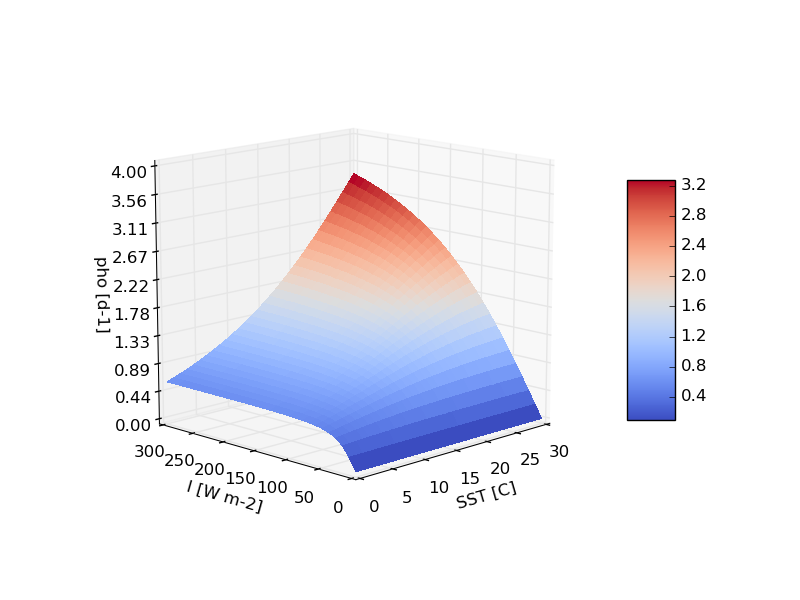
\includegraphics[scale=.66,trim=0.03cm 2cm 0cm 3cm,clip]{limf.png}}
	\caption{Combined light- \& temperature limitation function for the average phytoplankton growth rate in HAMOCC}
\label{fig:lighttemplimf}
\end{figure}
\vspace{.5cm}
\begin{figure}[h!]%bt]
\myfloatalign%\centering
\captionsetup[subfigure]{labelformat=empty,justification=centering}
	\subfloat[pCO$_{\text{2,ocean}}$(Alk, DIC, SST, SSS) \text{[ppm]}]{
	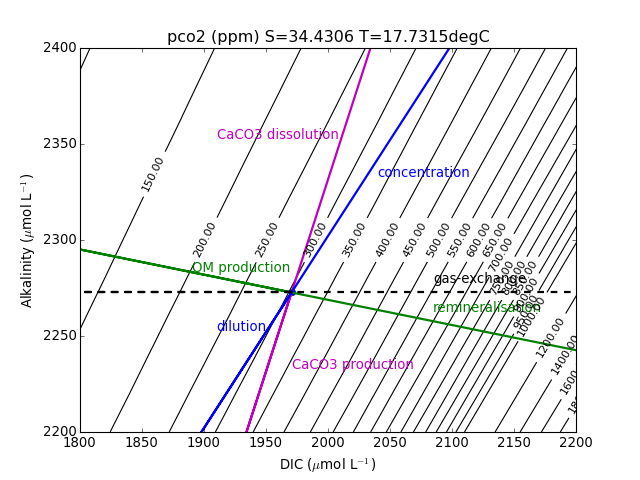
\includegraphics[scale=.63,trim=0.0cm 0cm 0cm 0cm,clip]{dic_alk_pco2_processes.png}}
	\caption{Deffeyes diagram and process contributions}
\label{fig:deffeyes_processes}
\end{figure}

%https://tex.stackexchange.com/questions/85776/change-figure-numbering-for-appendix

